\paragraph{Definition}
A continuous random variable is said to have a $F$-distribution with
$\nu_{1}$ et $\nu_{2}$ degrees of freedom if its probability density
function is of the form:
$$
f(x,\nu_{1},\nu_{2})=
\left\{
\begin{array}{ll}
	\dfrac{\Gamma\left(\frac{\nu_{1}+\nu_{2}}{2}\right)\left(\frac{\nu_{1}}{\nu_{2}}\right)^{\frac{\nu_{1}}{2}}x^{\frac{\nu_{1}}{2}-1}}{\Gamma\left(\frac{\nu_{1}}{2}\right)\Gamma\left(\frac{\nu_{2}}{2}\right)\left(1+\frac{\nu_{1}}{\nu_{2}}x\right)^{\left(\frac{\nu_{1}+\nu_{2}}{2}\right)}} & \mbox{if } 0\leq x < \infty\\
	0 & \mbox{otherwise}
\end{array}
\right.
$$
The $F$-distribution was named in honor of Sir Ronald Fisher by George
Snedecor. $F$-distribution arises as the distribution of a ratio of 
variances.
\begin{figure}[H]
	\begin{center}
		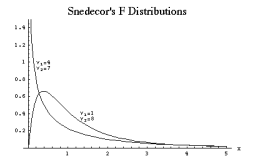
\includegraphics[width=.5\textwidth]{./chaps/23sec/images/2Snedecor_F_distribution.png}
	\end{center}
	\caption{Shape of the graph of $F$-distribution for various degrees of freedom.}
	\label{fig:23sec_F_distribution}
\end{figure}
\paragraph{Properties}
\subparagraph{Expected value and Variance}
$X\hookrightarrow F(\nu_{{1},nu_{2}})\Rightarrow$
$$
E(X) = 
\left\{
\begin{array}{ll}
	\frac{nu_{2}}{nu_{2}-2} & \mbox{if }\nu_{2}\geq 3 \\
	DNE &\mbox{if }\nu_{2}\in\inter{1}{2}
\end{array}
\right.
$$
\begin{center}
	And
\end{center}
$$
V(X) = 
\left\{
\begin{array}{ll}
	\frac{2\nu_{2}^{2}(\nu_{1}+\nu_{2}-2)}{\nu_{1}(\nu_{2}-2)^{2}(\nu_{2}-4)} & \mbox{if }\nu_{2}\geq 5 \\
	DNE &\mbox{if }\nu_{2}\in\inter{1}{4}
\end{array}
\right.
$$
\subparagraph{Inverse}
$X\hookrightarrow F(\nu_{1},\nu_{2})\Rightarrow \frac{1}{X}\hookrightarrow F(\nu_{2},\nu_{1})$\\
\subparagraph{Chi-squared and $F$-distributions}
$
\begin{cases}
	U\hookrightarrow\chi_{2}(\nu_{1})\\
	V\hookrightarrow\chi_{2}(\nu_{2})\\
	U\& V independent
\end{cases}
\Rightarrow
\dfrac{\frac{U}{\nu_{1}}}{\frac{V}{\nu_{2}}}\hookrightarrow F(\nu_{1},\nu_{2})
$
\subparagraph{Quotient of Inverses}
Let $X\hookrightarrow N(\mu_{1},\sigma_{1}^{2})\text{ and }\prth{X}{i}{1}{n}$ be a random sample of size $n$ from the population $X$.
Let $Y\hookrightarrow N(\mu_{2},\sigma_{2}^{2})\text{ and }\prth{Y}{i}{1}{m}$ be a random sample of size $n$ from the population $Y$.
$$
\dfrac{\frac{S_{1}^{2}}{\sigma_{1}^{2}}}{\frac{S_{2}^{2}}{\sigma_{2}^{2}}} \hookrightarrow F(n-1, m-1)
$$
where $S_{1}^{2}$, and $S_{2}^{2}$ denote the sample variances of the
first and second sample, respectively.
